\documentclass[12pt]{article}
\usepackage[pdftex]{graphicx}

\oddsidemargin  -0.5 cm
\evensidemargin 0.0 cm
\textwidth      6.5in
\headheight     0.0in
\topmargin      -1 cm
\textheight=9.0in

\begin{document}

\section{Light Charginos to Two Jets, One Lepton}

\begin{figure}[t]
  \begin{center}
    \begin{tabular}{p{0.49\linewidth} p{0.49\linewidth}}
      \begin{minipage}{\linewidth} \begin{center} Electrons left-polarized 95\% \end{center} \end{minipage} &
      \begin{minipage}{\linewidth} \begin{center} Electrons right-polarized 95\% \end{center} \end{minipage} \\
      \begin{minipage}{\linewidth} 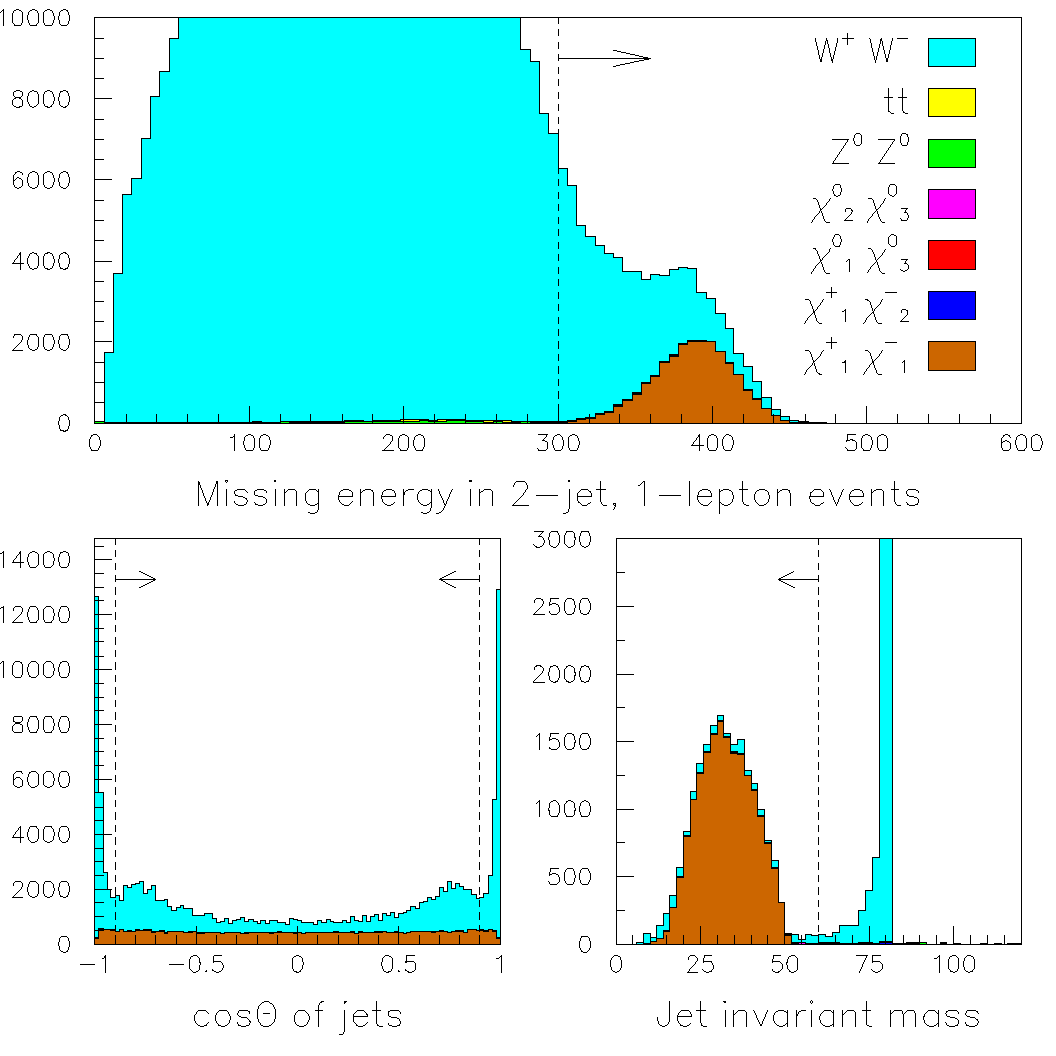
\includegraphics[width=\linewidth]{jimpcharginocuts_a} \end{minipage} &
      \begin{minipage}{\linewidth} 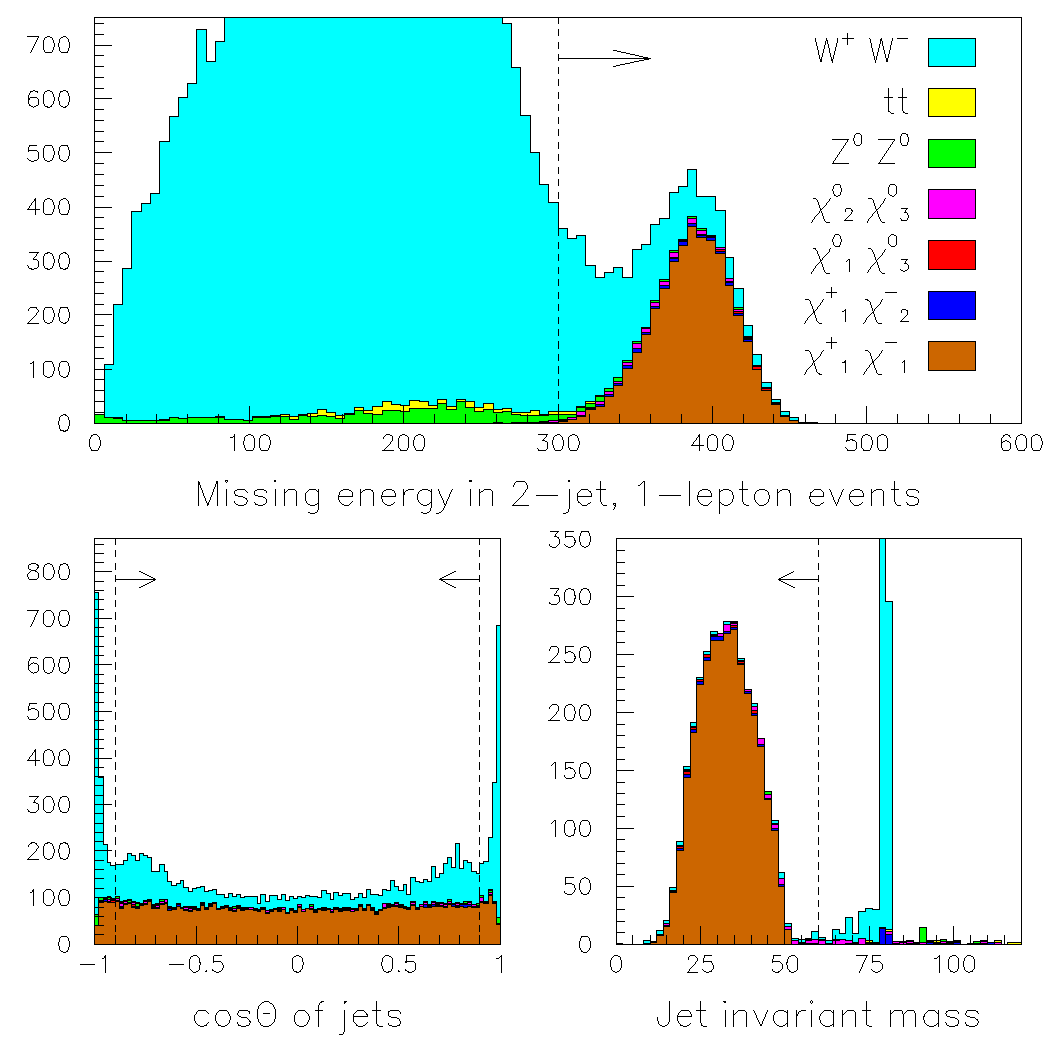
\includegraphics[width=\linewidth]{jimpcharginocuts_b} \end{minipage}
    \end{tabular}

    \caption{Event selection for light charginos from 250 fb$^{-1}$ of
    $e^+e^-$ collisions: the left set of plots have electrons 95\%
    left-polarized and the right set have electrons 95\% right
    polarized; positrons are unpolarized in both.  Within each set,
    the top plot is the missing energy for events with two jets and
    one lepton.  Bottom-left: $\cos\theta$ distribution of each jet
    where $\theta$ is the polar angle, with $>$ 300 GeV missing
    energy.  Bottom-right: Invariant mass of the two jets with missing
    energy and $|\cos\theta| >$ 0.9.  SUSY charginos are distinguished
    from Standard Model W-pairs by requiring the invariant mass to be
    $<$ 60 GeV.}

    \label{jimpcharginocuts}
  \end{center}
\end{figure}

\begin{center}
  \begin{tabular}{l l l l l l l}
    $e^+e^- \to $ & $\tilde{\chi}^+_1$ & & & $\tilde{\chi}^-_1$ & & \\
    & $\tilde{\chi}^+_1$ & $\to \tilde{\chi}^0_1$ & $W^+$ & $\tilde{\chi}^-_1$ & $\to \tilde{\chi}^0_1$ & $W^-$ \\
    & & & $W^+ \to jj$ & & & $W^- \to \ell^- \bar{\nu}$ \\
  \end{tabular}
\end{center}

\bigskip

The light chargino mode ($\tilde{\chi}^+_1 \tilde{\chi}^-_1$) is the
most copious of the four SUSY decays studied, and can be very cleanly
separated from all backgrounds by requiring two jets, exactly one
isolated track, and missing energy.  Each $\tilde{\chi}^\pm_1$ decays
into a $\tilde{\chi}^0_1$ and a virtual $W^\pm$, one $W^\pm$ decays
into two jets and the other into an electron or muon, and a neutrino.
The two ground-state neutralinos disappear as missing energy (along
with the neutrino), and the single lepton tags the event as the decay
of a pair of charged particles through $W^\pm$.  The invariant mass of
the two jets may then be used to veto Standard Model on-shell W
bosons, and then measure the $\tilde{\chi}^\pm_1$, $\tilde{\chi}^0_1$
mass difference by identifying the upper threshold.  Since the initial
state energy is known and the charginos can be cleanly separated from
all backgrounds, the absolute mass of the LSP $\tilde{\chi}^0_1$
can be estimated from the kinematic envelope of the two jets.

Two polarization states were studied: one in which the electrons are
95\% left-polarized and another in which the electrons are 95\%
right-polarized, with unpolarized positrons in either case.  After
requiring two distinguishable jets and an isolated track, identified
as a lepton, we require events to have more than 300 GeV of missing
energy.  At this point, the only significant background is Standard
Model W-pairs.  We further reject events in which either jet points
within 25 degrees of the beamline ($|\cos\theta| >$ 0.9 for polar
angle $\theta$), so that all of the energy and momentum of each jet is
accounted for.  Then we plot the invariant mass of the two jets, and
reject the peak from on-shell W-pairs by requiring the invariant mass
to be less than 60 GeV.  All of these selection criteria are presented
in Figure \ref{jimpcharginocuts}.

With these cuts, the sum of all physics backgrounds constitutes about
5--8\% of the measured events, so even after background subtraction,
the uncertainty in the number of chargino events seen can be taken to
be approximately the square root of this number.  With $\sigma$,
$\mathcal{L}$, $\mathcal{B}$, and $\varepsilon$ as the light chargino
cross-section, integrated luminosity, branching fraction to our final
state, and the efficiency of the cuts, respectively, the number of
events after cuts ($\sigma\mathcal{L}\mathcal{B}\varepsilon$) has
uncertainty $\sqrt{\sigma\mathcal{L}\mathcal{B}\varepsilon}$.
Therefore, the cross-section has uncertainty
\begin{equation}
  \sigma \pm \sqrt{\frac{\sigma}{\mathcal{L}\mathcal{B}\varepsilon}}.
\end{equation}
The product $\mathcal{B}\varepsilon$ is 7.7\% for charginos produced
with left-handed electrons and 10.5\% for charginos produced with
right-handed electrons, so the uncertainty in these cross-section
measurements scale as
\begin{equation}
  \sigma_L = 940\mbox{ fb} \pm \sqrt{\frac{940\mbox{ fb}}{0.077 \, \mathcal{L}}}
  \mbox{\hspace{0.5 cm} and \hspace{0.5 cm}}
  \sigma_R = 119\mbox{ fb} \pm \sqrt{\frac{119\mbox{ fb}}{0.105 \, \mathcal{L}}}.
\end{equation}
With 250 fb$^{-1}$, $\sigma_L$ can be measured to $\pm$7.0 fb and
$\sigma_R$ can be measured to $\pm$2 fb.

\begin{figure}[t]
  \begin{center}
    \begin{tabular}{p{0.49\linewidth} p{0.49\linewidth}}
      \begin{minipage}{\linewidth} 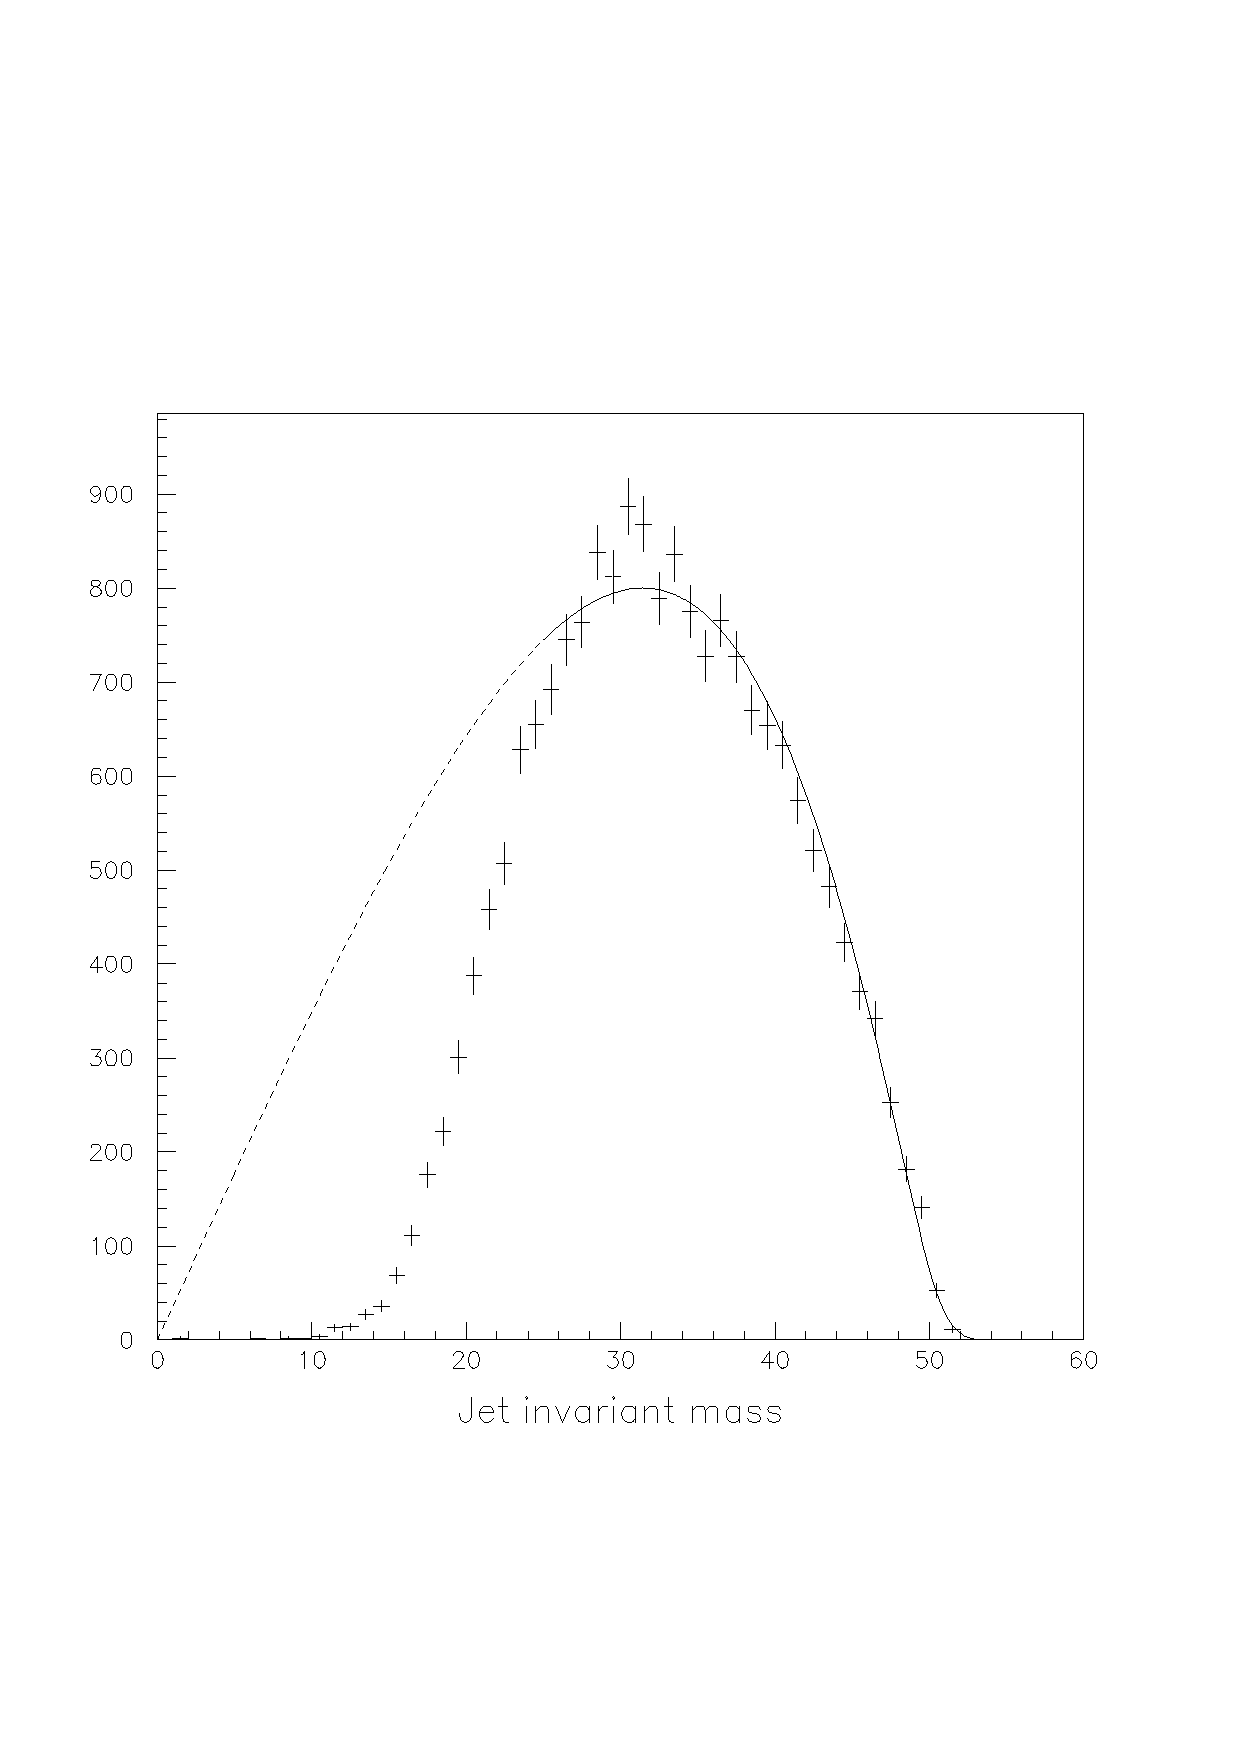
\includegraphics[width=\linewidth]{jimpcharginoanal_a} \end{minipage} &
      \begin{minipage}{\linewidth} 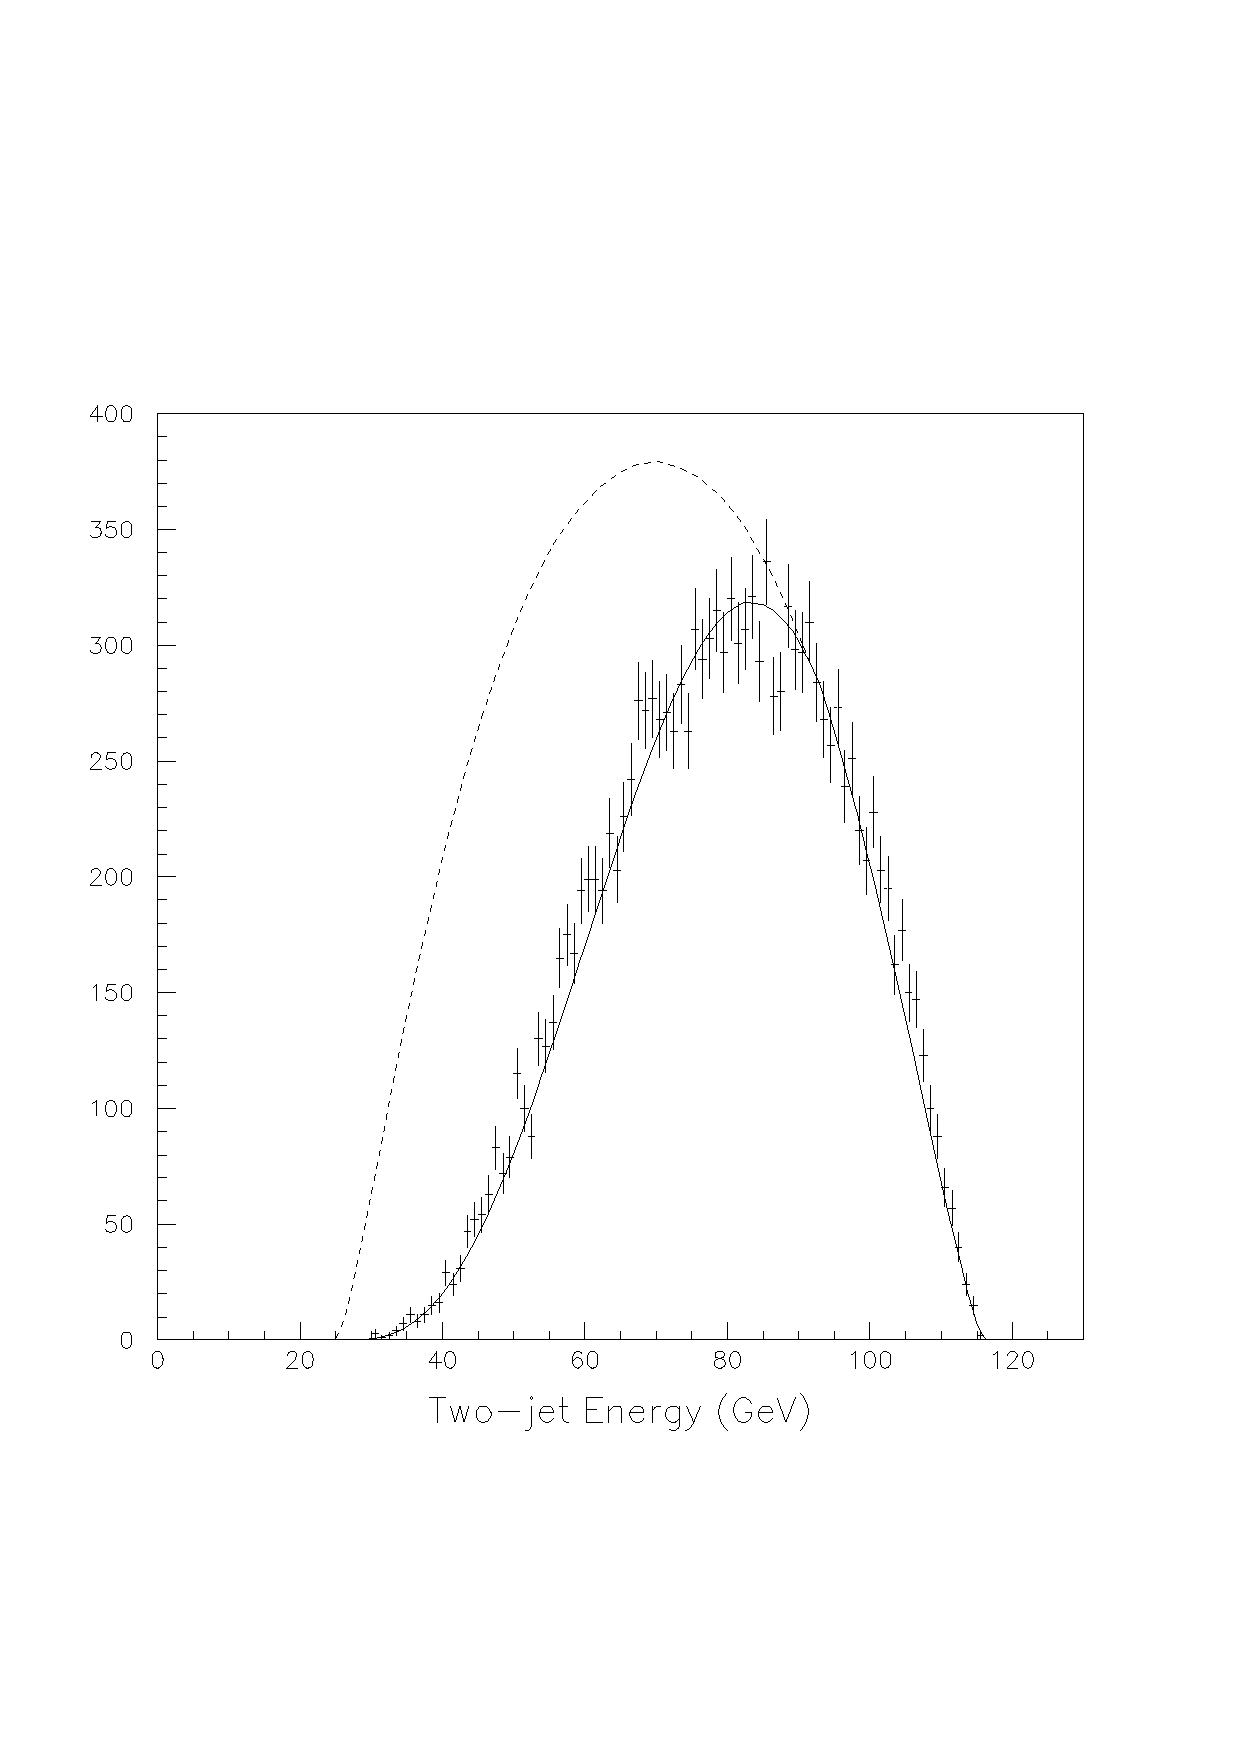
\includegraphics[width=\linewidth]{jimp_jetenergyfit} \end{minipage}
    \end{tabular}
    \caption{Light charginos from 250 fb$^{-1}$ of $e^+e^-$ collisions
    with electrons 95\% left-polarized and positrons unpolarized.
    Left: Maximum liklihood fit to two-jet invariant mass above 25 GeV
    (not efficiency corrected).  Right: Maximum liklihood fit to
    two-jet total energy (with invariant mass above 25 GeV).  The
    dotted line is the raw spectrum, and the solid line is efficiency
    corrected.}
    \label{jimpcharginoanal}
  \end{center}
\end{figure}

The upper threshold in the two jet invariant mass can be used to
measure the mass difference between $\tilde{\chi}^\pm_1$ and
$\tilde{\chi}^0_1$.  We proceed by fitting the left-polarized jet
invariant mass to the function described in section \ref{W}, which,
for our purposes, has two free parameters: the desired mass difference
and $\zeta = (|C_V|^2 - |C_A|^2)/(|C_V|^2 + |C_A|^2)$.  Anticipating a
sensitivity to bin spacing, we perform an unbinned maximum liklihood
fit to this function, with Gaussian smearing to adequately represent
mismeasured jets that lie above threshold.  A Gaussian smearing width
of 1.2 GeV is taken from the width of the real $W^\pm$ peak.  (Noting
the asymmetry in the $W^\pm$ peak from Figure \ref{jimpcharginocuts},
this convolution would be improved with a low-invariant mass tail.)
Invariant masses below 25 GeV are dropped from the fit, since pairs of
jets with low invariant masses are likely to overlap, leading to low
jet-finding efficiency.  From this fit, we obtain an uncertainty in
mass difference of $\pm$0.3 GeV and an $\zeta$ of 0.95 $\pm$0.02.
(See the left of Figure \ref{jimpcharginoanal}.)

While the invariant mass distribution is insensitive to the absolute
mass of $\tilde{\chi}^0_1$, this value can be obtained from the sum of
the jet energies.  The right of Figure \ref{jimpcharginoanal} shows
this distribution fitted to a curve derived from the invariant mass
distribution (keeping the mass difference fixed).  The jet energies
distribution needs to be corrected for initial state radiation, which
shifts the peak down 10 GeV, and it needs to be efficiency corrected,
as the jet efficiency is noticibly poor even above the peak.  The
high-energy edge of this plot (which is corrected for initial state
radiation and efficiency the least) is a function of
$\tilde{\chi}^0_1$ mass, the $\tilde{\chi}^\pm_1$-$\tilde{\chi}^0_1$
mass difference, and the lowest invariant mass events.  Since the
jet-finding efficiency is low for low invariant mass events, we again
restrict ourselves to events with invariant masses above 25 GeV, and
we fix the mass difference using the previous fit result.  An unbinned
maximum liklihood fit to the jet energies distribution yields a
$\pm$0.4 GeV statistical error in the $\tilde{\chi}^0_1$ mass, with
$\pm$0.5 GeV systematic error from uncertainty in the mass difference
and $\pm$0.2 GeV from uncertainty in $\zeta$.  This sets the mass
scale for the entire SUSY spectrum.

\end{document}
